
\subsection{Magic3D}\label{magic3D}

Magic3D represents a significant advancement in the domain of high-resolution 3D model generation from text input. Developed by \citeauthor{lin2023magic3d}, this method overcomes limitations observed in previous models like DreamFusion, particularly in terms of optimization speed and resolution of the generated models.

The core technique employed by Magic3D involves a coarse-to-fine optimization process. Initially, a coarse model is generated using a low-resolution diffusion prior, which is then fine-tuned in the second stage to yield a high-quality textured 3D mesh model \citep{lin2023magic3d}. This approach allows Magic3D to generate detailed 3D models with enhanced texture quality in a comparatively shorter time frame.

\begin{figure}[ht]
  \centering
    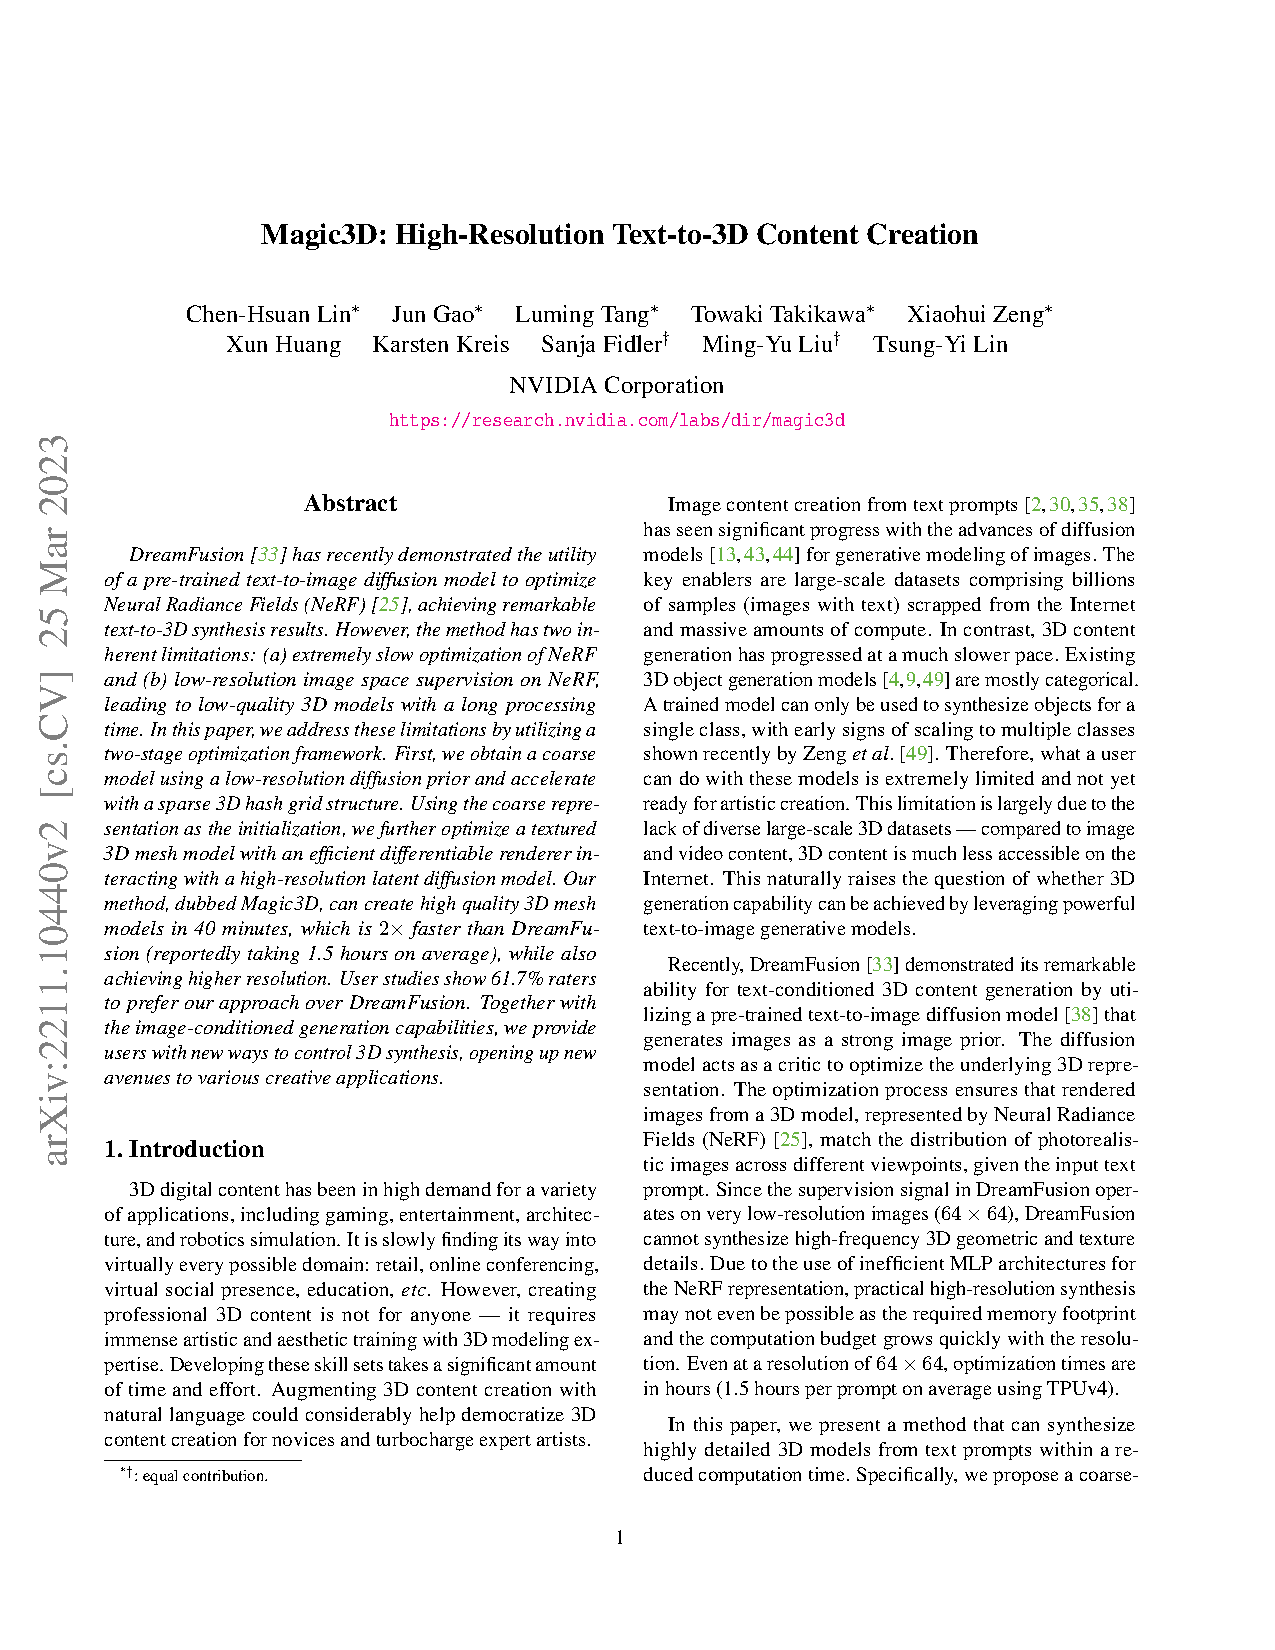
\includegraphics[width=1\columnwidth]{figures/Magic3D.png}
    \caption{This illustration from \citep{lin2023magic3d} showcases the Magic3D process, beginning with the InstantNGP for initial 3D representation. It then details the coarse-to-fine procedure, evolving to a refined high-resolution 3D mesh model.}\label{fig:figureMagic}
\end{figure}


Magic3D's process of generating 3D models from text prompts begins with an initial stage that employs the eDiff-I base diffusion model \citep{balaji2022eDiff-I}, akin to Google's Imagen \citep{saharia2022imagen}. This model operates at a relatively low resolution of \(64 \times 64\), laying the groundwork for the 3D geometry and textures given from the text input \citep{lin2023magic3d}. During this phase, the model uses a sparse 3D hash grid structure from Instant NGP \citep{mueller2022instant}, ``which allows us to represent high-frequency details at a much lower computational cost''~\citep{lin2023magic3d}. The optimization in this phase is performed by two single-layer neural networks that predict albedo (the base color of the object), density (how solid or transparent parts of the object are), and normals (which determine how light bounces off the surface) of the object \citep{lin2023magic3d}. This approach not only speeds up the optimization process but also ensures the foundational quality of the coarse 3D model \citep{lin2023magic3d}. 
This stage involves sampling an image from the NGP representation, which is then infused with an initial state of noise through the image diffusion prior. This step sets the stage for iterative refinement. The refinement is guided by the Score Distillation Sampling (\(L_{SDS}\)) loss function, which evaluates and compares the generated image against a target image, enabling the model to iteratively improve its accuracy. The use of the image diffusion prior in this low-resolution phase is primarily for shaping the overall structure and layout of the model, focusing more on broad features rather than fine details.

In the refinment stage, Magic3D focuses on refining this coarse model into a high-resolution textured mesh, marking a transition from the basic structure to a detailed representation. The refinement process starts with a 3D mesh derived from a deformable tetrahedral grid, where each grid vertex contains a value indicating its distance from the surface (signed distance field) and its deformation from the original position \citep{shen2021DMTet, lin2023magic3d}. The process begins by sampling a new image from this 3D mesh. This image is then processed by an encoder, which converts it into a format suitable for further processing by the latent diffusion model. The latent diffusion model used here, particularly Stable Diffusion \citep{rombachStableDiffusion}, operates at a high resolution of \(512 \times 512\), allowing for more detail of the final model \citep{lin2023magic3d}. Once the latent diffusion prior has processed the image, its output is evaluated using the Score Distillation Sampling \(L_{SDS}\) loss function. This function compares the generated image with a target image, enabling the model to fine-tune each vertex's signed distance field and deformation \citep{lin2023magic3d}. A technique employed here is the increase in focal length to zoom in on object details, essential for recovering high-frequency details in both geometry and texture \citep{lin2023magic3d}. Finally, the mesh is extracted using a differentiable marching tetrahedra algorithm, essential for achieving fine texturing \citep{lin2023magic3d}.

Magic3D's proficiency is not limited to just creating high-quality 3D models; it also offers extensive creative control over the generation process. The model supports ``fine-tuning a learned coarse model with a new prompt'' \citep{lin2023magic3d}, allowing users to influence the generated output significantly. This includes text-based edits and image-conditioned generation, increasing the scope for creative and personalized 3D model generation \citep{lin2023magic3d}.